\chapter{Des modes de quantité de mouvement aux champs quantiques}

Qu’est-ce qu’un champ quantique, et quel est son lien avec les particules ? L’outil mathématique de base est l’oscillateur harmonique. Un champ comporte de nombreux modes d’oscillation possibles ; quantifier le champ revient à associer un oscillateur harmonique quantique à chaque mode. La construction se voit plus facilement dans un premier temps dans un espace périodique fini, où les modes autorisés forment une liste discrète.

\section{Espace périodique et nombres d’onde autorisés}

Prenons une coordonnée spatiale \(x\) et identifions les points séparés par une distance \(L\). On peut se représenter l’espace comme un cercle de circonférence \(L\). C’est une astuce utile pour travailler à volume fini. Sur un intervalle fini avec des extrémités, une onde progressive se réfléchit aux bords. Sur un intervalle périodique, elle peut se propager dans un sens ou dans l’autre sans réflexion. La symétrie de translation, et donc la conservation de la quantité de mouvement, sont préservées tandis que l’on écarte temporairement les difficultés liées au volume infini.

Une onde plane s’écrit
\begin{equation}
e^{ikx}.
\end{equation}
Après un tour complet du cercle, elle doit retrouver sa valeur initiale. Comme l’onde vaut \(1\) en \(x=0\), la périodicité impose
\begin{equation}
e^{ikL}=1.
\end{equation}
Pourquoi un multiple entier de \(2\pi\) satisfait-il cette condition ? La formule d’Euler donne
\begin{align}
e^{i2\pi n}
&=\cos(2\pi n)+i\sin(2\pi n)\\
&=1,
\qquad n\in\mathbb Z.
\end{align}
Le cosinus vaut \(1\) et le sinus \(0\) après un nombre entier de cycles. Par conséquent,
\begin{equation}
kL=2\pi n,
\qquad
k=\frac{2\pi n}{L},
\qquad n\in\mathbb Z.
\end{equation}
La quantité \(k\) est le nombre d’onde. L’entier \(n\) repère un nombre d’onde autorisé ; il ne compte pas encore les particules.

On peut aussi exprimer la même condition en fonction de la longueur d’onde. Une longueur d’onde est la distance parcourue lorsque la phase avance d’un cycle complet, donc
\begin{equation}
k\lambda=2\pi,
\qquad
k=\frac{2\pi}{\lambda}.
\end{equation}
Une grande longueur d’onde correspond à un petit nombre d’onde, et une courte longueur d’onde à un grand nombre d’onde. La condition de périodicité signifie qu’un nombre entier de longueurs d’onde tient sur le cercle.

Pour une onde de mécanique quantique, la quantité de mouvement vaut
\begin{equation}
p=\frac{h}{\lambda}
=\frac{2\pi\hbar}{\lambda}
=\hbar k.
\end{equation}
Ainsi, \(k\) et \(p\) ne diffèrent que d’un facteur \(\hbar\). Les valeurs positives et négatives de \(k\) décrivent des ondes qui se propagent en sens opposés et des particules dont les quantités de mouvement sont orientées en sens opposés. Dans un système d’unités où \(\hbar=1\), on appelle couramment \(k\) la quantité de mouvement, sans autre distinction.

Pour chaque valeur autorisée de \(k\), ce mode peut contenir un certain nombre de quanta. Cela introduit un deuxième entier :
\begin{equation}
n(k)=\text{number of quanta with wave number }k.
\end{equation}
On l’appelle le nombre d’occupation. L’entier dans \(k=2\pi n/L\) repère le mode ; \(n(k)\) indique combien de particules occupent ce mode. Il faut spécifier les nombres d’occupation pour les valeurs négatives comme pour les valeurs positives de \(k\).

\begin{classroomqa}
\lecturetimestamp{00:11:58}
\audiencequestion{\(k\) est-il lui-même un entier ?}
\lecturerresponse{Non. Le nombre d’onde est un multiple entier de \(2\pi/L\) : \(k=2\pi n/L\). L’entier \(n\) dans cette formule repère la quantité de mouvement autorisée ; il est distinct du nombre d’occupation \(n(k)\), qui compte les quanta dans le mode.}
\end{classroomqa}

\section{États à nombre d’occupation et opérateurs de mode}

Un état quantique est un vecteur, ou un élément linéaire. On peut additionner les vecteurs d’état et les multiplier par des nombres ; les opérateurs agissent sur eux pour produire d’autres vecteurs d’état. Les quantités réelles observables sont représentées par des opérateurs hermitiens. Ces notions élémentaires sont importantes ici, car l’état à plusieurs particules comme le champ seront construits à partir de combinaisons linéaires et d’opérateurs.

Soit
\begin{equation}
k_j=\frac{2\pi j}{L},
\qquad j\in\mathbb Z.
\end{equation}
Une façon commode de désigner un état à plusieurs particules consiste à donner toute la suite des nombres d’occupation. En notant \(n_j\equiv n(k_j)\) les termes affichés, écrivons
\begin{equation}
\big|\{n(k_j)\}\big\rangle
=
\big|\ldots,n_{-2},n_{-1},n_0,n_1,n_2,\ldots\big\rangle.
\end{equation}
Le terme \(n(k_1)\) indique le nombre de particules dans le premier mode à quantité de mouvement positive, \(n(k_2)\) le nombre dans le deuxième, et ainsi de suite. La suite se prolonge indéfiniment dans les deux sens.

\begin{figure}[t]\centering
\includegraphics[width=0.72\textwidth]{lecture_03_figure_02.png}\caption{Nombre d’occupation \(n(k)\)}\lectureframe{00:15:04}\end{figure}

Chaque mode de quantité de mouvement est un oscillateur harmonique. Il possède donc un opérateur de montée et un opérateur de descente. La notation initialement écrite \(a^{+}(k)\) et \(a^{-}(k)\) sera remplacée par \(a^\dagger(k)\) et \(a(k)\). Leur action est la suivante :
\begin{align}
a^\dagger(k)\big|\ldots,n(k),\ldots\big\rangle
&=
\sqrt{n(k)+1}\notag\\
&\quad{}\times
\big|\ldots,n(k)+1,\ldots\big\rangle,
\\
a(k)\big|\ldots,n(k),\ldots\big\rangle
&=
\sqrt{n(k)}\,
\big|\ldots,n(k)-1,\ldots\big\rangle.
\end{align}
L’opérateur \(a^\dagger(k)\) agit sur la case correspondant à \(k\), augmente ce nombre d’occupation d’une unité et multiplie l’état par \(\sqrt{n(k)+1}\). L’opérateur \(a(k)\) diminue le nombre d’occupation dans la même case et fournit le facteur \(\sqrt{n(k)}\). Il existe une telle paire pour chaque quantité de mouvement autorisée.

\begin{figure}[t]\centering
\includegraphics[width=0.58\textwidth]{lecture_03_figure_03.png}\caption{Opérateurs de création et d’annihilation associés au mode de quantité de mouvement \(k\)}\lectureframe{00:17:14}\end{figure}

\section{Les coefficients de Fourier deviennent des opérateurs}

Le lien entre ces opérateurs d’oscillateur et un champ commence par une série de Fourier classique ordinaire. Un champ classique complexe sur l’intervalle périodique peut s’écrire
\begin{align}
\psi(x)&=\sum_k \alpha(k)e^{ikx},\\
\psi^*(x)&=\sum_k \alpha^*(k)e^{-ikx},
\end{align}
où chaque somme porte sur les valeurs autorisées \(k=2\pi n/L\). Cela revient à développer le champ en série de sinus et de cosinus.

Le champ complexe possède une partie réelle et une partie imaginaire. Son conjugué complexe inverse le signe de la partie imaginaire, et \(e^{ikx}\) devient \(e^{-ikx}\). La connaissance de tous les coefficients \(\alpha(k)\) détermine le champ classique. Il n’est pas nécessaire de spécifier \(\alpha^*(k)\) indépendamment dès lors que \(\alpha(k)\) est connu, mais les parties réelle et imaginaire de chaque coefficient sont deux quantités réelles distinctes. Elles peuvent être mesurées comme les amplitudes des composantes de Fourier correspondantes. En ce sens, un coefficient complexe regroupe deux observables classiques.

La quantification remplace ces coefficients de Fourier classiques par des opérateurs. Un signe d’égalité ordinaire identifierait des objets de natures différentes ; il est donc préférable d’écrire une règle de remplacement :
\begin{equation}
\alpha(k)\rightsquigarrow a(k),
\qquad
\alpha^*(k)\rightsquigarrow a^\dagger(k).
\end{equation}
Avec un choix cohérent des signes de Fourier, les champs quantiques sont définis par
\begin{align}
\Psi(x)&=\sum_k a(k)e^{ikx},\\
\Psi^\dagger(x)&=\sum_k a^\dagger(k)e^{-ikx}.
\end{align}\editorialnote{La discussion orale modifie, puis remet en question, la convention de signe de Fourier. La paire conjuguée utilisée ici correspond à la convention visible dans le développement du champ le plus clair et dans le calcul sur les états de position : \(\Psi\) porte le facteur \(e^{ikx}\) et \(\Psi^\dagger\) porte le facteur \(e^{-ikx}\). Inverser tous les signes de manière cohérente décrirait la même construction.}

Pour l’instant, il s’agit d’une définition : un champ quantique est une série de Fourier dont les coefficients sont des opérateurs. Pour justifier plus complètement cette définition, il faudrait montrer comment ces opérateurs reproduisent les coefficients classiques dans une limite appropriée, ce qui nécessite de considérer une certaine dynamique. Cette question est reportée à plus tard. On voit déjà que le champ lui-même est un opérateur et que les relations entre ses coefficients de Fourier sont celles des opérateurs de création et d’annihilation des oscillateurs harmoniques.

\begin{classroomqa}\lecturetimestamp{00:26:48}\audiencequestion{L’introduction des opérateurs de création et d’annihilation signifie-t-elle que la dynamique crée et détruit nécessairement des particules ?}
\lecturerresponse{Non. Ces opérateurs sont des opérations mathématiques qui modifient les nombres d’occupation. La question de savoir si les lois de la nature changent effectivement le nombre de particules relève de la dynamique. Si celle-ci permet de tels changements, ces opérateurs fournissent le langage naturel pour les décrire.}\end{classroomqa}

\section{Diffusion et nombre variable de particules}

Considérons d’abord un processus qui ne change pas le nombre de particules. Supposons que la seule particule présente initialement ait une quantité de mouvement \(k_7\). En notation des nombres d’occupation, son état comporte un \(1\) dans la septième case et des zéros partout ailleurs :
\begin{equation}
|k_7\rangle
=
|\ldots,0,\underset{k_7}{1},0,\ldots\rangle.
\end{equation}
Un processus de diffusion fait passer sa quantité de mouvement de \(k_7\) à \(k_9\). L’opérateur qui effectue exactement ce changement est
\begin{equation}
a^\dagger(k_9)a(k_7).
\end{equation}
L’opérateur le plus à droite agit en premier : il enlève la particule de la case \(k_7\). L’opérateur de gauche crée ensuite une particule dans la case \(k_9\).

\begin{classroomqa}\lecturetimestamp{00:31:37}\audiencequestion{Dans ce processus \(k_7\to k_9\), d’où viennent les facteurs de racine carrée ?}
\lecturerresponse{Le facteur d’annihilation est \(\sqrt{n(k_7)}=\sqrt{1}=1\). Après cette annihilation, le système se trouve dans l’état où toutes les occupations sont nulles. Comme le mode \(k_9\) est vide, le facteur de création est \(\sqrt{n(k_9)+1}=\sqrt{1}=1\). Dans cet exemple à une particule, aucun de ces facteurs ne modifie donc le coefficient numérique.}\end{classroomqa}

Effectuons les deux opérations. L’annihilation donne
\begin{align}
a(k_7)|k_7\rangle
&=
\sqrt{1}\,|\ldots,0,0,0,\ldots\rangle\\
&=|0\rangle.
\end{align}
L’état où toutes les occupations sont nulles est le vide. C’est l’état sans particule et, dans cet ensemble simple d’oscillateurs, c’est aussi l’état fondamental. La création dans le mode \(k_9\) vide donne alors
\begin{equation}
a^\dagger(k_9)|0\rangle
=\sqrt{0+1}\,|k_9\rangle
=|k_9\rangle.
\end{equation}
Par conséquent,
\begin{equation}
a^\dagger(k_9)a(k_7)|k_7\rangle=|k_9\rangle.
\end{equation}
Case par case, l’unique \(1\) est simplement passé du septième mode de quantité de mouvement au neuvième. Comme aucun nombre d’occupation n’a jamais dépassé un, les deux facteurs de racine carrée étaient égaux à un. Ils deviennent importants dès que l’on agit sur un mode déjà occupé.

Ce processus d’un à un pourrait aussi être décrit dans le cadre ordinaire de la mécanique quantique à une particule : une particule change de quantité de mouvement. Le langage des nombres d’occupation devient indispensable lorsque le nombre de particules peut varier. Par exemple,
\begin{equation}
a^\dagger(k_9)a^\dagger(k_{16})a(k_7)|k_7\rangle
=|k_9,k_{16}\rangle
\end{equation}
décrit le changement mathématique d’une particule incidente dans le mode \(k_7\) en deux particules sortantes, l’une dans le mode \(k_9\) et l’autre dans le mode \(k_{16}\). Une cible peut absorber la particule incidente, émettre les deux particules sortantes et subir le recul nécessaire. Un tel processus ne peut pas être représenté dans un espace de Hilbert limité à une particule, mais il s’inscrit naturellement dans un espace d’états où les nombres d’occupation peuvent varier. L’expression en opérateurs ne constitue pas à elle seule une loi de la nature ; elle fournit le langage dans lequel on peut écrire une loi qui change le nombre de particules.

\section{Un opérateur de champ en un point}

Que crée l’opérateur en représentation de position \(\Psi^\dagger(x)\) ? Les états quantiques forment un espace linéaire : on peut additionner des états de quantité de mouvement en les multipliant par des coefficients complexes pour former un nouvel état. Partons du vide. Comme tous les modes sont vides,
\begin{equation}
\Psi(x)|0\rangle=0.
\end{equation}
Le zéro à droite est le vecteur nul : un opérateur d’annihilation ne peut trouver aucune particule à enlever.

Le champ conjugué agit autrement :
\begin{align}
\Psi^\dagger(x)|0\rangle
&=\sum_k e^{-ikx}a^\dagger(k)|0\rangle\\
&=\sum_k e^{-ikx}|k\rangle,
\end{align}
où
\begin{equation}
|k\rangle=a^\dagger(k)|0\rangle
\end{equation}
est l’état à une particule de quantité de mouvement \(\hbar k\).

\begin{figure}[t]\centering
\includegraphics[width=0.70\textwidth]{lecture_03_figure_05.png}\caption{Développement de l’état formel en représentation de position \(\Psi^\dagger(x)|0\rangle\) sur les états de quantité de mouvement à une particule}\lectureframe{00:43:16}\end{figure}

Formellement, à un facteur de normalisation près, cette somme est l’état de position généralisé de la mécanique quantique à une particule.\footnote{Avec une infinité de modes de quantité de mouvement, un état de position parfaitement localisé n’est pas normalisable. En imposant une coupure de quantité de mouvement finie et en normalisant plutôt la somme tronquée, on obtient un paquet d’ondes fortement localisé autour de \(x\).} La combinaison des états propres de quantité de mouvement avec les coefficients \(e^{-ikx}\) produit une localisation en \(x\). En ce sens formel,
\begin{equation}
\Psi^\dagger(x)\ \text{creates a particle at position }x,
\end{equation}
tandis que
\begin{equation}
\Psi(x)\ \text{annihilates a particle at position }x.
\end{equation}
L’opérateur de mode \(a^\dagger(k)\) crée une particule de quantité de mouvement bien définie. L’opérateur de champ \(\Psi^\dagger(x)\) crée la superposition cohérente des états de quantité de mouvement autorisés qui est formellement localisée en \(x\).

Dans la somme formelle non normalisée, chaque coefficient \(e^{-ikx}\) a un module égal à un. Avec une coupure finie, l’état tronqué normalisé possède des coefficients de même module pour les quantités de mouvement retenues, tandis que leurs phases produisent un paquet d’ondes fortement localisé près de \(x\). C’est le lien élémentaire entre un champ quantique et les particules.

Pour l’instant, négligeons les complications de la relativité restreinte : dans ce modèle, \(\Psi^\dagger(x)\) crée une particule en \(x\). Les champs relativistes nécessitent des raffinements, mais le développement de Fourier à coefficients opérateurs ainsi que la distinction entre les opérateurs associés aux modes de quantité de mouvement et ceux en représentation de position restent fondamentaux.

\begin{classroomqa}\lecturetimestamp{00:44:59}\audiencequestion{\(x\) est-il un point du cercle périodique, et que se passe-t-il lorsque le cercle devient grand ?}
\lecturerresponse{Oui. Dans le modèle fini, \(x\) est un point du cercle. L’écart entre deux nombres d’onde autorisés voisins est \(2\pi/L\). Lorsque \(L\) augmente, cet écart diminue ; il existe donc, pour toute quantité de mouvement souhaitée, une valeur autorisée aussi proche que l’on veut. Dans la limite du volume infini, les sommes sur \(k\) sont remplacées par des intégrales sur \(k\). Il est utile de comprendre d’abord les sommes discrètes.}\end{classroomqa}

\section{Réactions locales entre particules}

Une fois que \(\Psi(x)\) et \(\Psi^\dagger(x)\) sont interprétés comme des opérateurs qui annihilent et créent des particules en un point, on peut exprimer directement la localité. Imaginons qu’une particule soit absorbée par une cible fortement localisée en \(x\), tandis qu’une particule sortante apparaît soudain près d’Alpha du Centaure et une autre près de Bételgeuse. Une telle réaction est non locale : ses événements éloignés ne peuvent pas être reliés par une propagation ordinaire.

On pourrait d’abord assouplir la condition et permettre aux particules sortantes d’être émises quelque part dans une petite région autour de la cible. L’idéalisation locale précise est plus forte : si la particule incidente est absorbée en \(x\), les particules sortantes sont créées en ce même point. Utiliser des champs évalués en des points distincts décrirait plutôt un produit d’opérateurs non local. Une opération locale d’une particule vers deux s’écrit donc
\begin{equation}
\Psi^\dagger(x)\Psi^\dagger(x)\Psi(x).
\end{equation}
Le champ le plus à droite enlève la particule incidente en \(x\) ; les deux champs à sa gauche y créent deux particules sortantes.\footnote{Le schéma local d’une réaction d’une particule vers deux suit la réaction décrite à 00:47:38--0049:13.}

\begin{figure}[t]\centering
\begin{tikzpicture}[scale=1.0]
\draw[->] (-2.2,0) -- (0,0);
\fill (0,0) circle (2.2pt);
\draw[->] (0,0) -- (2.0,1.1);
\draw[->] (0,0) -- (2.0,-1.1);
\node at (-1.25,0.3) {$k_{\mathrm{initial}}$};
\node[right] at (0.05,0.05) {$x$};
\node at (1.48,1.34) {$\ell$};
\node at (1.48,-1.34) {$m$};
\end{tikzpicture}\caption{Une particule incidente est absorbée en \(x\) et deux particules sortantes sont créées au même point.}\end{figure}

Supposons que l’état incident contienne une particule de nombre d’onde bien défini \(k_{\mathrm{initial}}\). Pour déterminer les quantités de mouvement sortantes, substituons les développements des champs en représentation de quantité de mouvement. Il importe de distinguer un indice de quantité de mouvement fixé d’un indice muet de sommation. Écrivons
\begin{align}
\Psi(x)&=\sum_q a(q)e^{iqx},\\
\Psi^\dagger(x)&=\sum_\ell a^\dagger(\ell)e^{-i\ell x}.
\end{align}
L’indice \(q\) est muet, tandis que \(k_{\mathrm{initial}}\) repère le mode incident particulier occupé. Les deux occurrences de \(\Psi^\dagger(x)\) nécessitent elles aussi des indices muets indépendants, par exemple \(\ell\) et \(m\). Réutiliser un même indice lierait à tort deux sommes indépendantes. Ici, \(\ell\) et \(m\) sont des nombres d’onde ; \(m\) ne désigne pas une masse.

On peut se représenter concrètement un photon frappant un atome localisé en \(x\), puis deux photons quittant ce point. Le champ simple utilisé ici convient mieux aux particules non relativistes qu’à un champ photonique pleinement relativiste ; le langage des photons ne sert donc qu’à illustrer le calcul avec les opérateurs.

Le champ d’annihilation agit en premier :
\begin{align}
\Psi(x)|k_{\mathrm{initial}}\rangle
&=\sum_q e^{iqx}a(q)a^\dagger(k_{\mathrm{initial}})|0\rangle.
\end{align}
Tous les termes s’annulent, sauf celui pour lequel \(q=k_{\mathrm{initial}}\). Un opérateur d’annihilation doit trouver une particule dans son propre mode. On obtient donc
\begin{equation}
\Psi(x)|k_{\mathrm{initial}}\rangle
=e^{ik_{\mathrm{initial}}x}|0\rangle.
\end{equation}
Les deux champs de création donnent ensuite
\begin{align}
&\Psi^\dagger(x)\Psi^\dagger(x)\Psi(x)
|k_{\mathrm{initial}}\rangle
\\
&\quad=
e^{ik_{\mathrm{initial}}x}
\sum_{\ell,m}
e^{-i\ell x}e^{-imx}
a^\dagger(\ell)a^\dagger(m)|0\rangle
\\
&\quad=
\sum_{\ell,m}
e^{i(k_{\mathrm{initial}}-\ell-m)x}
a^\dagger(\ell)a^\dagger(m)|0\rangle.
\end{align}
Si \(\ell\) et \(m\) sont distincts, on peut noter l’état opérateur \(|\ell,m\rangle\) : un mode est occupé par une particule, et l’autre aussi. Le résultat final est une somme sur toutes ces configurations de quantité de mouvement à deux particules, avec une phase déterminée par les quantités de mouvement incidente et sortantes.

\begin{classroomqa}\lecturetimestamp{01:00:36}\audiencequestion{Les deux opérateurs de création commutent-ils ?}
\lecturerresponse{Oui. Tous les opérateurs de création commutent entre eux, de même que tous les opérateurs d’annihilation. Un opérateur de création et un opérateur d’annihilation commutent lorsqu’ils se rapportent à des modes différents ; pour un même mode, leur commutateur est non nul.}\end{classroomqa}

\begin{classroomqa}\lecturetimestamp{01:01:34}\audiencequestion{Les quantités de mouvement des deux particules sortantes doivent-elles respecter la conservation de la quantité de mouvement ?}
\lecturerresponse{Les particules représentées n’ont pas à conserver à elles seules la quantité de mouvement, car l’atome ou la cible peut subir un recul. La différence \(k_{\mathrm{initial}}-\ell-m\) est la quantité de mouvement transférée à la cible. C’est la quantité de mouvement totale, cible comprise, qui est conservée.}\end{classroomqa}

Comme le coefficient \(e^{i(k_{\mathrm{initial}}-\ell-m)x}\) est une phase pure, son module vaut un. À première vue, cela semble indiquer des poids de probabilité égaux pour toutes les paires \((\ell,m)\). Il faut toutefois apporter une réserve importante lorsque les deux indices coïncident.

Si \(\ell=m\), le premier opérateur de création place une particule dans le mode \(m\), puis le second agit sur un mode déjà occupé une fois :
\begin{align}
a^\dagger(m)a^\dagger(m)|0\rangle
&=a^\dagger(m)|1_m\rangle\\
&=\sqrt{2}\,|2_m\rangle.
\end{align}
La création de deux particules dans un même mode comporte donc un facteur d’amplitude supplémentaire \(\sqrt{2}\). Le carré d’une amplitude fait apparaître un facteur \(2\) dans la probabilité.

\begin{classroomqa}\lecturetimestamp{01:04:54}\audiencequestion{Faut-il que \(\ell\) et \(m\) diffèrent d’une unité parce que le coefficient de création contient \(n+1\) ?}
\lecturerresponse{Non. Les symboles \(\ell\) et \(m\) repèrent des modes de quantité de mouvement. Le \(n\) dans \(\sqrt{n+1}\) est le nombre d’occupation du mode particulier sur lequel agit l’opérateur de création. Les indices de quantité de mouvement et les nombres de particules sont des entiers distincts.}\end{classroomqa}

\begin{figure}[t]\centering
\includegraphics[width=0.92\textwidth]{lecture_03_figure_06.png}\caption{Développement en représentation de quantité de mouvement de l’amplitude locale d’une réaction d’une particule vers deux}\lectureframe{01:05:44}\end{figure}

Les particules de cette construction sont identiques. Le facteur \(\sqrt{2}\) est donc un facteur d’occupation bosonique ; il ne sert pas à distinguer une première particule d’une seconde. En élevant ce facteur au carré, il semble, à titre provisoire, que l’issue où les quantités de mouvement sont égales soit deux fois plus probable qu’un terme où elles diffèrent. Il faudra réexaminer cette comparaison après avoir compté soigneusement les termes de la double somme.

\begin{classroomqa}\lecturetimestamp{01:06:43}\audiencequestion{Dans une réaction complexe, comment choisit-on l’ordre des opérateurs de création et d’annihilation ?}
\lecturerresponse{Une expression où tous les opérateurs de création sont à gauche et tous les opérateurs d’annihilation à droite est dite normalement ordonnée. Sous cette forme, les opérateurs les plus à droite enlèvent d’abord les particules incidentes, puis les opérateurs restants créent les particules sortantes.}\end{classroomqa}

La réorganisation d’une paire composée d’un opérateur de création--et d’un opérateur d’annihilation n’est généralement pas une simple permutation : elle fait intervenir le commutateur, qui produit un terme supplémentaire pour un même mode.\footnote{Cette précision sur le commutateur corrige la discussion informelle de l’ordre normal à 01:06:43.}

\begin{classroomqa}\lecturetimestamp{01:07:30}\audiencequestion{Si les amplitudes associées aux quantités de mouvement ont toutes le même module, que signifie une affirmation comme « ``deux fois plus probable'' » ?}
\lecturerresponse{Gardons à l’esprit la cavité finie. Ses quantités de mouvement autorisées sont discrètes, ce qui permet de comparer les probabilités mode par mode. La comparaison ne porte pas sur les probabilités de points isolés dans un continuum.}\end{classroomqa}

Pour \(\ell\ne m\), la double somme sans restriction contient les deux termes ordonnés
\begin{equation}
a^\dagger(\ell)a^\dagger(m)|0\rangle
\quad\text{and}\quad
a^\dagger(m)a^\dagger(\ell)|0\rangle.
\end{equation}

\begin{classroomqa}\lecturetimestamp{01:08:24}\audiencequestion{Lorsque \(\ell\ne m\), le même état final apparaît-il deux fois dans la double somme, une fois sous la forme \((\ell,m)\) et une fois sous la forme \((m,\ell)\) ?}
\lecturerresponse{Oui. Si \(\ell\ne m\), les termes \((\ell,m)\) et \((m,\ell)\) apparaissent tous deux et, puisque les opérateurs de création commutent, ils décrivent le même état physique.}\end{classroomqa}

Les deux termes ordonnés étant égaux, il faut tenir compte de la normalisation des états et de ce double comptage avant d’effectuer une comparaison quantitative entre les canaux. La conclusion algébrique sûre est plus restreinte, mais elle suffit pour la suite : créer une particule dans un mode déjà occupé par \(n\) bosons identiques produit le facteur \(\sqrt{n+1}\).

\section{Émission spontanée et émission stimulée}

Un exemple plus simple permet d’isoler le facteur de racine carrée. Supposons qu’un objet localisé en \(x\) émette un photon. Si le champ photonique est initialement dans le vide, l’état sortant est
\begin{align}
\Psi^\dagger(x)|0\rangle
&=\sum_k e^{-ikx}a^\dagger(k)|0\rangle\\
&=\sum_k e^{-ikx}|k\rangle.
\end{align}
Dans ce modèle simplifié, le module des amplitudes est le même pour toutes les quantités de mouvement. En l’absence de photons préexistants, l’émission est spontanée.

Supposons maintenant qu’un photon soit déjà présent dans le mode \(\ell\). Le même champ de création produit deux types de termes :
\begin{equation}
\Psi^\dagger(x)|\ell\rangle
=
\sum_{k\ne\ell}e^{-ikx}|k,\ell\rangle
+e^{-i\ell x}\sqrt{2}\,|2_\ell\rangle.
\end{equation}
Pour \(k\ne\ell\), l’opérateur crée dans un mode vide, de sorte que le coefficient vaut \(\sqrt{0+1}=1\). Pour \(k=\ell\), il crée dans le mode occupé, de sorte que le coefficient vaut \(\sqrt{1+1}=\sqrt{2}\). Le photon initial ne subit aucune action ; le nouveau photon est émis de préférence dans le mode déjà occupé.

\begin{classroomqa}\lecturetimestamp{01:16:14}\audiencequestion{Le photon préexistant doit-il se trouver au même endroit pour stimuler l’émission ?}
\lecturerresponse{Le calcul simplifié porte sur l’occupation d’un même mode de quantité de mouvement, et non sur deux particules situées en une position parfaitement définie. Une particule ne peut avoir à la fois une position et une quantité de mouvement exactes. Les photons réels sont décrits par des paquets d’ondes, tandis que l’idéalisation de la cavité fournit des modes discrets bien définis. Dans ce cadre, l’émission est renforcée dans le mode de cavité déjà occupé.}\end{classroomqa}

Si le mode \(\ell\) contient initialement \(n_\ell\) photons, alors
\begin{equation}
a^\dagger(\ell)
|\ldots,n_\ell,\ldots\rangle
=
\sqrt{n_\ell+1}
\,|\ldots,n_\ell+1,\ldots\rangle.
\end{equation}
La probabilité est donc accrue d’un facteur \(n_\ell+1\). Avec un photon déjà présent, ce facteur vaut \(2\). Si le mode contient cent photons, le facteur d’amplitude est \(\sqrt{101}\) et la probabilité d’émission dans ce mode est \(101\) fois supérieure à celle d’un mode vide. Plus un mode bosonique contient déjà de quanta, plus il est probable que le quantum suivant soit émis dans ce mode. C’est l’émission stimulée.

Le même effet lié à l’occupation apparaît dans les réactions de diffusion. Si une collision peut produire une particule dans plusieurs modes, une occupation préexistante favorise la production dans les modes occupés. C’est une propriété générale de cette algèbre des oscillateurs, et non une particularité de la désintégration atomique.

\begin{classroomqa}\lecturetimestamp{01:18:15}\audiencequestion{Dans le processus précédent à deux particules, les deux particules nouvellement créées ont-elles encore un poids plus élevé lorsque leurs quantités de mouvement diffèrent ?}
\lecturerresponse{Oui. Dans la double somme ordonnée, une paire de quantités de mouvement inégales apparaît dans deux ordres. Le facteur de même mode \(\sqrt{2}\) réduit cette différence combinatoire, mais ne la supprime pas à lui seul.}\end{classroomqa}

Comme précédemment, toute comparaison entre canaux physiques exige une normalisation cohérente des états et un décompte cohérent.

\begin{classroomqa}\lecturetimestamp{01:18:30}\audiencequestion{Cela signifie-t-il que les bosons sont attirés vers les états de quantité de mouvement déjà occupés ?}
\lecturerresponse{Non. Il n’y a ni force ni attraction au sens littéral. Ce renforcement est une conséquence statistique de l’identité des particules et des facteurs de racine carrée dans les opérateurs de création bosoniques.}\end{classroomqa}

Il est utile de distinguer les deux termes. En l’absence de photons, le coefficient commence par \(n=0\), ce qui donne le facteur unité associé à l’émission spontanée. Si des photons sont déjà présents, le facteur \(n+1\) rend plus probable l’émission dans leur mode ; c’est l’émission stimulée.

Il existe un analogue classique. Une onde électromagnétique préexistante qui passe près d’un atome met ses électrons en mouvement. Ceux-ci rayonnent alors plus fortement qu’en l’absence de l’onde, et le rayonnement supplémentaire suit la direction et le nombre d’onde de l’onde excitatrice. L’énoncé quantique remplace l’onde préexistante par des modes photoniques occupés : les quanta déjà présents stimulent la production d’autres quanta dans le même mode.

Les particules régies par cette algèbre des oscillateurs sont des bosons. Elles ont une tendance statistique à s’accumuler dans les états occupés, sans pour autant s’attirer vers ces états. Il existe deux types de statistique pour les particules : les bosons et les fermions. La construction présentée ici est bosonique ; le comportement fermionique opposé sera étudié plus loin.

\section{Algèbre bosonique et densité de particules}

À chaque mode de quantité de mouvement correspondent des opérateurs de création et d’annihilation. Leur algèbre est
\begin{align}
[a^\dagger(k),a^\dagger(\ell)]&=0,\\
[a(k),a(\ell)]&=0,\\
[a(k),a^\dagger(\ell)]&=\delta_{k\ell}.
\end{align}
Ici,
\begin{equation}
[A,B]=AB-BA,
\end{equation}
et le delta de Kronecker est défini par
\begin{equation}
\delta_{k\ell}=
\begin{cases}
1,&k=\ell,\\
0,&k\ne\ell.
\end{cases}
\end{equation}
Les opérateurs de création commutent entre eux, que leurs quantités de mouvement soient égales ou non, et il en va de même pour les opérateurs d’annihilation. Une paire mixte commute pour des quantités de mouvement différentes ; pour une même quantité de mouvement, elle vérifie le commutateur familier de l’oscillateur harmonique simple.

Avec la définition de Fourier de \(\Psi(x)\), ces relations définissent le champ quantique bosonique le plus simple. Le champ sert à créer et à annihiler des particules, mode par mode ou en des positions données.

Considérons maintenant l’opérateur
\begin{equation}
\int_0^L dx\,\Psi^\dagger(x)\Psi(x).
\end{equation}
Plutôt que de lui donner d’emblée un nom, calculons-le. En substituant les développements de Fourier, on obtient
\begin{align}
\int_0^L dx\,\Psi^\dagger(x)\Psi(x)
&=
\sum_{k,\ell}a^\dagger(k)a(\ell)
\int_0^L dx\,e^{-ikx}e^{i\ell x}
\\
&=
\sum_{k,\ell}a^\dagger(k)a(\ell)
\int_0^L dx\,e^{i(\ell-k)x}.
\end{align}
Si \(k=\ell\), l’exponentielle vaut \(1\) et l’intégrale vaut \(L\). Si \(k\ne\ell\), on intègre sur le cercle un nombre entier de périodes du sinus et du cosinus ; les parties positives et négatives se compensent. Ainsi,
\begin{equation}
\int_0^L dx\,e^{i(\ell-k)x}=L\delta_{k\ell}.
\end{equation}
La double somme se réduit à
\begin{equation}
\int_0^L dx\,\Psi^\dagger(x)\Psi(x)
=L\sum_k a^\dagger(k)a(k).
\end{equation}
Pour chaque mode,
\begin{equation}
a^\dagger(k)a(k)=N_k
\end{equation}
est l’opérateur nombre d’occupation. Leur somme compte toutes les particules :
\begin{equation}
N=\sum_k N_k=\sum_k a^\dagger(k)a(k).
\end{equation}
Avec la normalisation de Fourier utilisée ici,
\begin{equation}
N=\frac{1}{L}\int_0^L dx\,
\Psi^\dagger(x)\Psi(x).
\end{equation}
D’autres conventions introduisent dans le développement de Fourier des facteurs tels que \(1/\sqrt{L}\), ce qui supprime le facteur explicite \(1/L\) ici. Dans la convention utilisée, l’opérateur local de densité de particules est
\begin{equation}
\rho(x)=\frac{1}{L}\Psi^\dagger(x)\Psi(x),
\qquad
\int_0^L dx\,\rho(x)=N.
\end{equation}
Ainsi, \(\Psi^\dagger(x)\Psi(x)\) est proportionnel à la densité de particules. Dire qu’il représente le nombre de particules en un point mathématique est trompeur ; la densité est la notion locale appropriée.

Le nombre total peut être conservé ou ne pas l’être. Si la dynamique crée ou absorbe des particules, \(N\) peut varier au cours du temps. Si la dynamique conserve le nombre de particules, alors \(N\) est une observable conservée.

La connaissance des commutateurs des opérateurs de mode permet également de calculer les commutateurs de \(\Psi(x)\) et \(\Psi^\dagger(x)\). Ce calcul est laissé comme exercice utile d’application des sommes de Fourier.

Cette construction décrit une espèce de bosons identiques. Identiques signifie que toutes les particules sont de même nature, même si elles peuvent avoir des positions et des impulsions différentes. On ne mettrait pas des électrons et des photons dans le même champ \(\Psi\). Un champ de photons nécessite des améliorations relativistes de ce modèle élémentaire. Un champ d’électrons requiert une algèbre différente, celle des fermions.

\begin{classroomqa}\lecturetimestamp{01:35:43}\audiencequestion{Cette construction est-elle propre à une seule dimension ?}\lecturerresponse{L’exemple considéré jusqu’ici comporte une seule coordonnée spatiale, mais rien d’essentiel ne dépend de cela. On passe à des dimensions supérieures en introduisant des coordonnées et des composantes de l’impulsion supplémentaires.}\end{classroomqa}

\editorialnote{Un bref échange semble commencer par évoquer la fluorescence et l’émission stimulée, puis aborder la transparence et les interférences. Le texte endommagé ne permet pas de reconstituer de façon fiable la question ni sa réponse.}

Parmi les exemples figurent les photons, le boson de Higgs et les gravitons.\footnote{Les autres noms de particules de cette brève liste d’exemples sont indistincts et ne sont pas repris.}

\section{Grande occupation et limite classique du champ}

Un opérateur de champ complexe n’est pas à lui seul une observable hermitienne. Ses deux composantes hermitiennes sont
\begin{equation}
\Psi_1(x)=\frac{\Psi(x)+\Psi^\dagger(x)}{2},
\quad
\Psi_2(x)=\frac{\Psi(x)-\Psi^\dagger(x)}{2i}.
\end{equation}
Elles sont les analogues quantiques des parties réelle et imaginaire d’un champ classique. Elles ne commutent pas ; on ne peut donc pas mesurer les deux simultanément avec une précision arbitraire. C’est, pour le champ, l’analogue de l’incertitude entre les variables conjuguées d’un oscillateur harmonique.

Dans quelles conditions le champ peut-il alors se comporter comme une onde classique ? Considérons un mode d’impulsion \(k\) fortement excité. Son opérateur nombre est
\begin{equation}
a^\dagger(k)a(k)=N_k.
\end{equation}
Supposons que l’état ait une occupation moyenne élevée, \(\langle N_k\rangle=n_k\gg 1\). L’échelle disponible pour l’amplitude d’un oscillateur macroscopique est alors de l’ordre de \(\sqrt{n_k}\). Pendant ce temps, le membre de droite de
\begin{equation}
[a(k),a^\dagger(k)]=1
\end{equation}
reste fixe. Le commutateur ne s’annule jamais, mais, à grande occupation, ses effets peuvent être faibles par rapport au carré de l’échelle de l’excitation. Une grande occupation fournit l’échelle nécessaire à une limite classique, mais ne suffit pas à elle seule. L’état doit aussi présenter une cohérence de phase appropriée, de sorte que les incertitudes des deux quadratures soient petites devant l’amplitude macroscopique du champ.\footnote{Cela précise l’heuristique de la grande occupation. Un état propre du nombre vérifie \(\langle a(k)\rangle=0\), n’a pas de phase définie et présente des fluctuations des quadratures de l’ordre de \(\sqrt{n_k}\) ; à lui seul, il ne constitue pas une onde classique.}

Pour un champ électromagnétique, une grande occupation signifie un grand nombre de photons. Dans un état présentant une cohérence de phase appropriée et contenant beaucoup de photons dans les modes pertinents, les composantes mesurables du champ se comportent approximativement comme une onde électromagnétique classique ordinaire. Avec seulement quelques photons, la discrétude des quanta devient visible et la description par une onde classique échoue. Dans les deux régimes, le champ quantique reste un opérateur ; c’est l’importance relative de ses fluctuations quantiques qui change.

\begin{classroomqa}\lecturetimestamp{01:42:09}\audiencequestion{Le grand nombre d’occupation correspond-il à l’occupation initiale ou à l’occupation finale ?}\lecturerresponse{Si le processus ne modifie que légèrement le nombre de photons, cela n’a pas d’importance pour cet argument. Les occupations initiale et finale sont toutes deux grandes, et leur différence est petite devant chacune d’elles.}\end{classroomqa}

À l’autre extrême se trouve l’état fondamental, dans lequel tous les nombres d’occupation sont nuls. Cet état est profondément quantique, et il faut soigneusement distinguer sa notation de celle du vecteur nul.

\begin{classroomqa}\lecturetimestamp{01:42:36}\audiencequestion{Si un opérateur d’annihilation agit sur le vide, produit-il de nouveau le vide, ou bien aucun état ?}\lecturerresponse{Il produit le vecteur nul, \(a(k)|0\rangle=\mathbf{0}\). Le vide \(|0\rangle\) est un véritable état normalisé sans particules, qui vérifie \(\langle0|0\rangle=1\). Ce n’est pas le vecteur nul. Le vecteur nul a une norme nulle et ne représente aucun état physique.}\end{classroomqa}

\begin{classroomqa}\lecturetimestamp{01:44:11}\audiencequestion{Le champ lui-même est-il une autre sorte d’état ?}\lecturerresponse{Non. En théorie quantique des champs, le champ est un opérateur. Les états sont des vecteurs, sur lesquels agissent les opérateurs de champ.}\end{classroomqa}

\section{L’espace périodique en pratique}

La construction périodique est un outil de calcul ; elle ne signifie pas que l’Univers soit littéralement un cercle d’une circonférence choisie. Des systèmes à modes discrets très semblables existent toutefois en pratique.

\begin{classroomqa}\lecturetimestamp{01:45:03}\audiencequestion{Comment utilise-t-on en pratique le modèle périodique fini ?}\lecturerresponse{Le rayonnement dans une cavité à parois réfléchissantes fournit un ensemble discret de modes bien connu. Une particule circulant dans un fil fermé en est un exemple directement périodique. Il n’est ni nécessaire ni particulièrement utile de prendre \(L\) pour taille de l’Univers.}\end{classroomqa}

Fixer \(L\) impose un écart non nul entre impulsions adjacentes, mais ne limite pas leur nombre.

\begin{classroomqa}\lecturetimestamp{01:45:39}\audiencequestion{Fixer la longueur \(L\) limite-t-il le nombre total d’états d’impulsion possibles ?}\lecturerresponse{Non. Les valeurs permises sont \(k_j=2\pi j/L\), et \(j\) peut être n’importe quel entier ; il reste donc une infinité de modes. Une valeur finie de \(L\) ne donne qu’un nombre fini de modes en dessous d’une impulsion maximale choisie. Sans une telle coupure, l’indice d’impulsion reste non borné.}\end{classroomqa}

On peut aussi lire à rebours l’interprétation en oscillateur. En mécanique élémentaire de l’oscillateur, on part de variables conjuguées pour construire \(a\) et \(a^\dagger\). Ici, les opérateurs de mode ont été introduits en premier ; il est donc naturel de se demander où apparaissent leurs variables conjuguées.

\begin{classroomqa}\lecturetimestamp{01:46:43}\audiencequestion{Pour un mode fixé, qu’est-ce qui correspond aux variables de l’oscillateur \(X\) et \(P\) lorsque la construction part de \(a(k)\) et \(a^\dagger(k)\) ?}\lecturerresponse{À chaque mode d’impulsion fixé correspond un oscillateur. Ses deux quadratures hermitiennes sont construites à partir de \(a(k)\) et \(a^\dagger(k)\), tout comme les composantes réelle et imaginaire du champ sont construites à partir de \(\Psi\) et \(\Psi^\dagger\). À un facteur de normalisation près et éventuellement en permutant les noms, elles sont les analogues de \(X\) et \(P\).}\end{classroomqa}

Pour le mode fixé, en omettant les facteurs numériques dépendant des conventions, les quadratures sont\footnote{L’échange à 01:46:43 passe assez librement d’un mode de quantité de mouvement au champ complet. La relation affichée explicite l’énoncé pour un mode fixé : \(\Psi(x)\) et \(\Psi^\dagger(x)\) sont des sommes de Fourier sur tous les modes.}\begin{equation}
X_k\propto a(k)+a^\dagger(k),
\qquad
P_k\propto \frac{a(k)-a^\dagger(k)}{i}.
\end{equation}
\(\Psi_1(x)\) et \(\Psi_2(x)\), les composantes en espace des positions introduites plus haut, sont des superpositions de Fourier de ces quadratures de mode, et non les quadratures d’un mode fixé. Leur relation d’incertitude exprime le même obstacle que celui rencontré lorsqu’on tente de considérer un champ quantique faiblement excité comme un objet entièrement classique.

\section{L’espace périodique en dimensions supérieures}

\begin{classroomqa}\lecturetimestamp{01:48:21}\audiencequestion{Comment représente-t-on l’espace périodique en plus d’une dimension ?}\lecturerresponse{En deux dimensions, l’analogue du cercle est un tore. On peut le représenter par un rectangle dont les bords gauche et droit sont identifiés, ainsi que les bords inférieur et supérieur. Il y a deux directions périodiques, donc les deux composantes de l’impulsion sont quantifiées.}\end{classroomqa}

On représente souvent un tore comme la surface d’un beignet, mais un rectangle est plus pratique pour les calculs. On découpe la surface une première fois et on l’ouvre pour obtenir un cylindre. On découpe ensuite le cylindre une nouvelle fois et on l’aplatit. Le rectangle obtenu conserve deux identifications : le bord gauche correspond au bord droit, et le bord inférieur au bord supérieur.\footnote{01:48:46--01:50:58. Le rectangle, ses deux identifications de bords, la réapparition de la particule et l’énoncé selon lequel les deux composantes de l’impulsion sont quantifiées découlent de ce passage. Les formules affichées pour \(k_x\) et \(k_y\) sont la reconstruction composante par composante de la condition antérieure \(kL=2\pi n\).}

Une particule qui franchit le bord droit réapparaît au point correspondant du bord gauche. Si elle franchit le bord supérieur, elle réapparaît au point correspondant du bord inférieur. Un champ périodique vérifie
\begin{align}
\Psi(x+L_x,y)&=\Psi(x,y),\\
\Psi(x,y+L_y)&=\Psi(x,y).
\end{align}
Pour une onde plane \(e^{i(k_x x+k_y y)}\), ces identifications imposent
\begin{equation}
k_x=\frac{2\pi n_x}{L_x},
\qquad
k_y=\frac{2\pi n_y}{L_y},
\qquad
n_x,n_y\in\mathbb Z.
\end{equation}
Les deux composantes de l’impulsion sont discrètes.

\begin{figure}[t]\centering
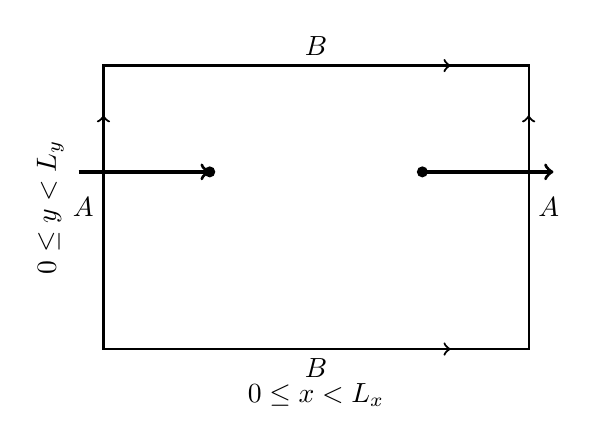
\begin{tikzpicture}[x=0.9cm,y=0.9cm]
\draw[thick] (0,0) rectangle (6,4);
\draw[->,thick] (0,0.7) -- (0,3.3);
\draw[->,thick] (6,0.7) -- (6,3.3);
\draw[->,thick] (1.1,0) -- (4.9,0);
\draw[->,thick] (1.1,4) -- (4.9,4);
\node[left] at (0,2) {$A$};
\node[right] at (6,2) {$A$};
\node[below] at (3,0) {$B$};
\node[above] at (3,4) {$B$};
\draw[->,very thick] (4.5,2.5) -- (6.35,2.5);
\draw[->,very thick] (-0.35,2.5) -- (1.5,2.5);
\fill (4.5,2.5) circle (2pt);
\fill (1.5,2.5) circle (2pt);
\node at (3,-0.65) {$0\leq x<L_x$};
\node[rotate=90] at (-0.75,2) {$0\leq y<L_y$};
\end{tikzpicture}\caption{Espace périodique bidimensionnel : les bords portant la même étiquette sont identifiés, de sorte qu’une particule qui franchit un bord réapparaît au point correspondant du bord opposé.}\end{figure}

\begin{classroomqa}\lecturetimestamp{01:50:58}\audiencequestion{La construction périodique représente-t-elle l’espace ou les objets qui s’y trouvent ?}\lecturerresponse{Elle représente l’espace. Les objets et les champs y sont définis et respectent ses identifications. On impose la périodicité pour maîtriser le problème en volume infini ; on la supprime en faisant tendre le volume vers de grandes valeurs et en remplaçant les sommes sur les impulsions par des intégrales.}\end{classroomqa}

L’analogue tridimensionnel est un cube dont les trois paires de faces opposées sont identifiées. Les faces gauche et droite correspondent l’une à l’autre, tout comme les faces supérieure et inférieure, ainsi que les faces avant et arrière. Une particule qui franchit une face réapparaît par la face qui lui est identifiée.\footnote{01:51:27--01:52:17. Le cube périodique et ses trois paires de faces identifiées découlent de ce passage. L’équation affichée pour \(k_i\) est la reconstruction composante par composante de la condition antérieure \(kL=2\pi n\), appliquée aux trois directions périodiques.} Les trois composantes de l’impulsion vérifient
\begin{equation}
k_i=\frac{2\pi n_i}{L_i},
\qquad i=x,y,z,
\end{equation}
avec un entier \(n_i\) pour chaque direction. On peut définir des tores en toute dimension selon la même règle.

\begin{figure}[t]\centering
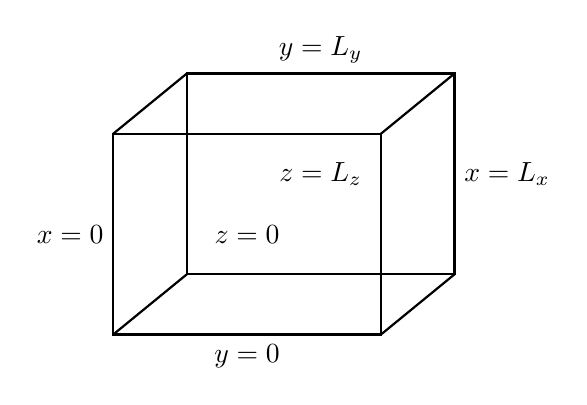
\begin{tikzpicture}[scale=0.85]
\draw[thick] (0,0) rectangle (4,3);
\draw[thick] (1.1,0.9) rectangle (5.1,3.9);
\draw[thick] (0,0) -- (1.1,0.9);
\draw[thick] (4,0) -- (5.1,0.9);
\draw[thick] (4,3) -- (5.1,3.9);
\draw[thick] (0,3) -- (1.1,3.9);
\node[left] at (0,1.5) {$x=0$};
\node[right] at (5.1,2.4) {$x=L_x$};
\node[below] at (2,0) {$y=0$};
\node[above] at (3.1,3.9) {$y=L_y$};
\node at (2,1.5) {$z=0$};
\node at (3.1,2.4) {$z=L_z$};
\end{tikzpicture}\caption{Espace périodique tridimensionnel représenté par un cube dont chaque paire de faces opposées est identifiée.}\end{figure}

\begin{classroomqa}\lecturetimestamp{01:52:20}\audiencequestion{La théorie des champs attribue-t-elle une taille physique au maillage de l’espace ?}\lecturerresponse{C’est une question spéculative. Pour les besoins de la présente discussion, l’espace est continu. Les quanta sont des particules, et non des cellules d’un maillage spatial. Dans la construction du cercle, c’est l’impulsion qui devient discrète ; la position reste continue et périodique.}\end{classroomqa}

\editorialnote{Un long passage endommagé au cours de l’échange sur la taille du maillage mentionne des échelles de Planck, mais ne conserve aucune affirmation reconstituable sur une discrétude fondamentale de l’espace. Aucune affirmation de ce type n’est déduite ici.}

La discrétude de \(k\) provient entièrement de l’imposition d’une fonction d’onde périodique. Elle ne prouve pas que la coordonnée \(x\) elle-même soit définie sur un réseau. Il est légitime de se demander si l’espace possède une structure microscopique fondamentale, mais c’est une question distincte et spéculative.

\section{Fermions et champs externes}

Les modes bosoniques peuvent avoir n’importe quel nombre d’occupation entier non négatif. Pour les fermions, c’est le comportement opposé qui s’impose : le principe d’exclusion de Pauli interdit à deux fermions identiques d’occuper le même état.

\begin{classroomqa}\lecturetimestamp{01:55:13}\audiencequestion{La théorie fermionique la plus simple s’obtient-elle en remplaçant les commutateurs par des anticommutateurs ?}\lecturerresponse{Oui, pour l’essentiel. Le commutateur est \([A,B]=AB-BA\), tandis que l’anticommutateur est \(\{A,B\}=AB+BA\). L’algèbre fermionique correspondante de création et d’annihilation met en œuvre l’exclusion de Pauli : on ne peut pas ajouter un second fermion identique à un état déjà occupé. L’étude détaillée est reportée.}\end{classroomqa}

Les deux produits diffèrent par un signe :
\begin{equation}
[A,B]=AB-BA,
\qquad
\{A,B\}=AB+BA.
\end{equation}
Le commutateur est antisymétrique par échange, tandis que l’anticommutateur est symétrique. Si un anticommutateur s’annule, alors
\begin{equation}
\{A,B\}=0
\quad\Longrightarrow\quad
AB=-BA.
\end{equation}
Pour une telle paire, l’échange des deux opérateurs fermioniques change le signe. C’est plus inhabituel que la commutation ordinaire, où \([A,B]=0\) implique \(AB=BA\). Remplacer les commutateurs bosoniques par l’algèbre anticommutative correspondante est le changement mathématique qui conduit aux fermions ; son étude détaillée est reportée.

L’anticommutation inverse le comportement statistique observé pour les bosons. Les fermions identiques ne s’accumulent pas dans un même mode par émission stimulée ; l’occupation de ce mode empêche un autre fermion identique de s’y ajouter. Puisqu’un état fermionique donné ne peut contenir au plus qu’un fermion identique, on ne peut obtenir de limite de champ classique en en plaçant un nombre arbitrairement grand dans cet état unique.

\begin{classroomqa}\lecturetimestamp{01:58:03}\audiencequestion{Comment une particule alpha peut-elle être un boson si elle est constituée de fermions ?}\lecturerresponse{Un objet composite lié contenant un nombre pair de constituants fermioniques peut obéir à une statistique bosonique. Placer plusieurs de ces bosons composites dans le même état global n’équivaut pas à placer leurs constituants fermioniques individuels dans un même état à une particule.}\end{classroomqa}

La statistique composite concerne l’objet lié dans son ensemble. Des constituants fermioniques peuvent donc s’assembler pour former un objet qui se comporte comme un boson sans que le principe d’exclusion appliqué aux constituants soit violé.

\begin{classroomqa}\lecturetimestamp{01:58:33}\audiencequestion{Comment incorpore-t-on des champs externes ?}\lecturerresponse{Aucun champ de fond externe n’a été inclus jusqu’ici dans la construction. On peut prescrire un tel champ comme champ classique, ou le représenter en mécanique quantique par un état contenant un grand nombre de quanta.}\end{classroomqa}

Pour que les deux descriptions concordent, l’état à grande occupation doit être préparé de façon appropriée et présenter une cohérence de phase ; le seul nombre de particules ne suffit pas.\footnote{L’échange introduit l’échelle associée à un grand nombre de quanta. La cohérence de phase est énoncée ici comme la condition supplémentaire qui évite de confondre une grande occupation à elle seule avec un champ classique.} Dans ce régime semi-classique, leurs effets concordent à de faibles écarts quantiques près. Il s’agit d’une condition fondamentale de cohérence. Le champ électromagnétique doit décrire des photons discrets lorsque les quanta individuels comptent, tout en reproduisant l’action familière d’une onde électromagnétique classique dans un état approprié, cohérent en phase et contenant beaucoup de photons.